\documentclass[12pt, a4paper]{article}
\usepackage{amsmath}
\usepackage{enumitem}
\usepackage{float}
\usepackage[left=2cm, right=2cm, top=2cm, bottom=2cm]{geometry}
\usepackage{graphicx}
\usepackage[colorlinks, urlcolor=blue]{hyperref}
\usepackage{minted}
\usepackage{siunitx}
\usepackage{xeCJK}

\renewcommand\arraystretch{1.1}
\setCJKmainfont[AutoFakeBold=1.5]{新細明體}
\setlength{\parindent}{0pt}

\title{
  \vspace{-1cm}
  Network Administration/System Administration\\
  (NTU CSIE, Spring 2024)\\
  Homework \#10
}
\author{\Large B12902110 呂承諺}

\setminted{frame=single}

\begin{document}
  \maketitle
  \section{課程內容}
  \begin{enumerate}[label=(\alph*)]
    \item 5~GHz Wi-Fi uses frequencies ranging from \qty{5.15}{\giga\hertz} to
    \qty{5.35}{\giga\hertz} and \qty{5.47}{\giga\hertz} to \qty{5.895}{\giga\hertz}.
    We choose \qty{5.50}{\giga\hertz} as an average for calculation.
    \[
      \lambda = \frac{c}{f}
      = \frac{\qty{299792458}{\meter/\second}}{\qty{5.50e9}{Hz}}
      = \qty{0.0545}{\meter} = \qty{54.5}{\milli\meter}
    \]

    \item
    \[
      \frac{P_r}{P_t} = \frac{G_tG_r\lambda^2}{\left(4\pi d\right)^2}
      = \frac{1 \left(1\right) \left(0.0545\right)^2}{\left(4\pi \left(1\right) \right)^2}
      = \num{1.88e-5}
    \]

    \item For a certain wavelength $\lambda$, suppose only the distance changes, while
    all other factors remain the same.
    \[
      P_r = \frac{P_t G_t G_r \lambda^2}{\left(4 \pi d\right)^2} \propto \frac{1}{d^2}
    \]
    This shows that both 2.4~GHz and 5~GHz signals attenuate by the same factor.

    \item Suppose the wavelength is the only changing factor.
    \[
      P_r = \frac{P_t G_t G_r \lambda^2}{\left(4 \pi d\right)^2} \propto \lambda^2
    \]
    2.4~GHz waves have a longer wavelength than 5~GHz waves, so 2.4~GHz gets a stronger
    signal.

    \item Bandwidth refers to the maximum data transfer rate of the connection, while
    throughput refers to the actual data transfer rate.
  \end{enumerate}

  \textbf{References}
  \begin{footnotesize}
    \begin{itemize}
      \item \href{https://en.wikipedia.org/wiki/Wi-Fi}{Wi-Fi - Wikipedia}
      \item \href{https://en.wikipedia.org/wiki/List_of_WLAN_channels}{List of WLAN channels - Wikipedia}
      \item \href{https://en.wikipedia.org/wiki/Friis_transmission_equation}{Friis transmission equation - Wikipedia}
      \item \href{https://cool.ntu.edu.tw/courses/33591/files/5577514}{Lecture slides "Wireless Communications \& Networking" by Professor Michael Tsai, page 12}
      \item \href{https://en.wikipedia.org/wiki/Bandwidth_(signal_processing)}{Bandwidth (signal processing) - Wikipedia}
      \item \href{https://en.wikipedia.org/wiki/Bandwidth_(computing)}{Bandwidth (computing) - Wikipedia}
      \item \href{https://blog.pichuang.com.tw/20190527-bandwidth-and-throughput.html}{Bandwidth \& Throughput - 魂系架構 Phil's Workspace}
      \item \href{https://en.wikipedia.org/wiki/Network_throughput}{Network throughput - Wikipedia}
    \end{itemize}
  \end{footnotesize}

  \section{討論題}
  \begin{enumerate}[label=(\alph*)]
   \item
   \item
   \item
   \item
  \end{enumerate}

  \section{問答題}
  \begin{enumerate}[label=(\alph*)]
    \item SSID
    \begin{enumerate}[label=(\arabic*)]
      \item SSID stands for service set identifier. It is typically the network name that
      users see.

      BSSID stands for basic service set identifier. It is usually the MAC address of the
      access point.

      One extended service set (ESS), identified by an SSID, may consist of one or
      more access points. Each access point has its own BSSID.

      \item An AP can provide service of several SSIDs simultaneously. Most home APs today
      can deploy a main SSID and another guest SSID. Another example is using different SSIDs
      for 2.4~GHz and 5~GHz signals from the same AP.

      Different APs can share the same SSID. Just configure the APs to the same SSID. This is
      exactly how the \verb|csie| Wi-Fi works in the department.

      \item An evil twin is a malicious Wi-Fi AP that mimics a legitimate one, often
      set up to have the same SSID as a public Wi-Fi and a fake login page. When a device
      automatically connects to the AP, the attacker can start monitoring the victim's
      traffic and extract sensitive information.

      We can prevent the evil twin attack by not connecting to public or insecure
      Wi-Fi, and by using secure application protocols.

      \item The device will often choose the AP with the best signal quality or the first
      one that it connected to. Standards 802.11k, 802.11v, and 802.11r facilitate transition
      between basic service sets.
    \end{enumerate}
    \textbf{References}
    \begin{footnotesize}
      \begin{itemize}
        \item \href{https://en.wikipedia.org/wiki/Service_set_(802.11_network)}{Service set (802.11 network) - Wikipedia}
        \item \href{https://en.wikipedia.org/wiki/Evil_twin_(wireless_networks)}{Evil twin (wireless networks) - Wikipedia}
        \item \href{https://usa.kaspersky.com/resource-center/preemptive-safety/evil-twin-attacks}{What is an Evil Twin Attack? Evil Twin Wi-Fi Explained}
        \item \href{https://learn.microsoft.com/en-us/windows-hardware/drivers/network/fast-roaming-with-802-11k--802-11v--and-802-11r}{Fast Roaming with 802.11k, 802.11v, and 802.11r - Windows drivers | Microsoft Learn}
      \end{itemize}
    \end{footnotesize}

    \item I would place the new AP at the front-left of the classroom, as its the
    farthest to both existing APs.

    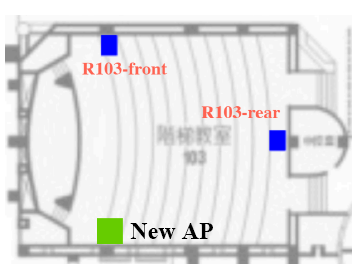
\includegraphics[width=0.5\textwidth]{3-b_new_ap.png}
  \end{enumerate}

  \section{實作題}
  \begin{enumerate}[label=(\alph*)]
    \item \textbf{Steps}
    \begin{enumerate}[label=(\arabic*)]
      \item If this is the first time connecting to the Wi-Fi, we need to create a profile in
      XML format. Here we use a WPA3-Personal profile as an example.
      \inputminted[fontsize=\footnotesize]{xml}{Ultramarine.xml}
      Then we add it to the system.
      \begin{Verbatim}[frame=single]
netsh wlan add profile filename=Ultramarine.xml
      \end{Verbatim}
      \item Connect to the Wi-Fi with the following command.
      \begin{Verbatim}[frame=single]
netsh wlan connect name=Ultramarine
      \end{Verbatim}
    \end{enumerate}
    \textbf{Result}

    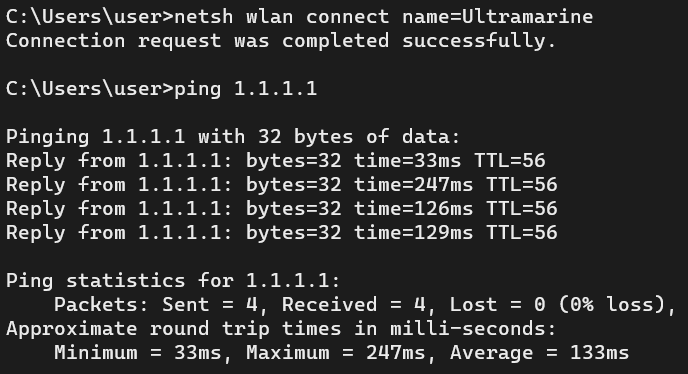
\includegraphics[width=0.6\textwidth]{4-a_netsh.png}

    \textbf{References}
    \begin{itemize}
      \item \href{https://www.windowscentral.com/how-connect-wi-fi-network-windows-10}{How to connect to a Wi-Fi network on Windows 10 | Windows Central}
      \item \href{https://stackoverflow.com/questions/32760356/how-to-connect-to-a-wifi-in-powershell-knowing-the-ssid-and-password}{How to connect to a wifi in powershell knowing the SSID and password? - Stack Overflow}
      \item \href{https://learn.microsoft.com/en-us/windows/win32/nativewifi/wpa2-personal-profile-sample}{WPA2-Personal profile sample - Win32 apps | Microsoft Learn}
    \end{itemize}

    \item \verb|csie| and \verb|csie-5g| both use WPA2-Enterprise, type PEAP. This can be seen
    in network properties in Windows' settings.

    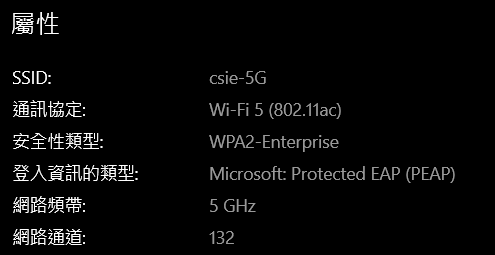
\includegraphics[width=0.5\textwidth]{4-b_csie-5G.png}
  \end{enumerate}
\end{document}
